\subsection{Zadania}

\setcounter{problem}{0}

\begin{problem}
  Policja w Nowym Yorku próbuje złapać przestępce znajdującego się w punkcie $\otimes$. Obstawiła część ulic, ale nie wszystkie. Przestępca w każdym korku porusza się losowo (tzn. z prawdopodobieństwem $1/4$ w każdym z możliwych kierunków). Jeżeli wpadnie na policję $\bullet$ zostaje złapany, jeżeli dotrze do jednego z pól $\circ$ ucieka. Oblicz prawdopodobieństwo, że uda mu się uciec.

  \begin{center}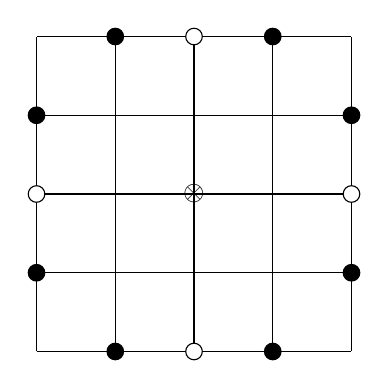
\begin{tikzpicture}
    \foreach \x in {0, ..., 4}
      {
        \draw(0,\x)--(4, \x);
        \draw(\x, 0)--(\x, 4);
      }

    \filldraw (0, 1) circle (3pt);
    \filldraw (0, 3) circle (3pt);
    \filldraw (1, 0) circle (3pt);
    \filldraw (3, 0) circle (3pt);
    \filldraw (3, 4) circle (3pt);
    \filldraw (1, 4) circle (3pt);
    \filldraw (4, 1) circle (3pt);
    \filldraw (4, 3) circle (3pt);
    \filldraw[fill=white] (0, 2) circle (3pt);
    \filldraw[fill=white] (4, 2) circle (3pt);
    \filldraw[fill=white] (2, 0) circle (3pt);
    \filldraw[fill=white] (2, 4) circle (3pt);

    \node at (2,2) {$\otimes$};
  \end{tikzpicture}\end{center}
\end{problem}

\begin{solution}
Zacznę od oznaczenia pozycji literkami:
\begin{center}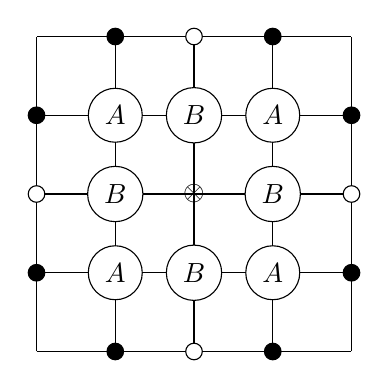
\begin{tikzpicture}[fun/.style={circle, color=black, fill=white, minimum size=3mm, draw=black, thin}]
    \foreach \x in {0, ..., 4}
      {
        \draw(0,\x)--(4, \x);
        \draw(\x, 0)--(\x, 4);
      }

    \filldraw (0, 1) circle (3pt);
    \filldraw (0, 3) circle (3pt);
    \filldraw (1, 0) circle (3pt);
    \filldraw (3, 0) circle (3pt);
    \filldraw (3, 4) circle (3pt);
    \filldraw (1, 4) circle (3pt);
    \filldraw (4, 1) circle (3pt);
    \filldraw (4, 3) circle (3pt);
    \filldraw[fill=white] (0, 2) circle (3pt);
    \filldraw[fill=white] (4, 2) circle (3pt);
    \filldraw[fill=white] (2, 0) circle (3pt);
    \filldraw[fill=white] (2, 4) circle (3pt);

    \node[fun] at (1, 1) {$A$};
    \node[fun] at (2, 1) {$B$};
    \node[fun] at (3, 1) {$A$};
    \node[fun] at (1, 2) {$B$};
    \node[fun] at (3, 2) {$B$};
    \node[fun] at (1, 3) {$A$};
    \node[fun] at (3, 3) {$A$};
    \node[fun] at (2, 3) {$B$};

    \node at (2,2) {$\otimes$};
  \end{tikzpicture}\end{center}
  oraz $\otimes$ jest oznaczone $S$, $\bullet$ to $0$ oraz $\circ$ będzie $1$. Niech $P_i$ oznacza prawdopodobieństwo ucieczki jeśli jesteśmy na polu $i$. Wtedy
  $$
    \begin{cases}
      P_S=\frac{1}{4}(P_B+P_B+P_B+P_B)=P_B\\ 
      P_B=\frac{1}{4}(P_1+P_S+P_A+P_A)=\frac{1}{4}(P_1+P_S)+\frac{1}{2}P_A\\ 
      P_A=\frac{1}{4}(P_B+P_B+P_0+P_0)=\frac{1}{2}(P_B+P_0)\\ 
      P_1=1\\ 
      P_0=0
    \end{cases}
  $$
  W takim razie $P_A=\frac{1}{2}P_B$ oraz
  $$
  P_B=\frac{1}{4}(1+P_S)+\frac{1}{4}P_B\implies 3P_B=1+P_S\implies 3P_B=1+P_B\implies P_B=\frac{1}{2}
  $$
  ale ponieważ $P_S=P_B$, to odpowiedź końcowa wynosi $\frac{1}{2}$.
\end{solution}

\begin{problem}
  Alicja i Robert rzucają symetryczną monetą tak długo aż wypadnie $OOOR$ lub $ORRR$. Alicja wygrywa, gdy wzorzec $OOOR$ wypadnie jako pierwszy, natomiast Robert, gdy wypadnie $ORRR$. Oblicz prawdopodobieństwo, że grę wygra Alicja.
\end{problem}

\begin{solution}
  Tak jak na wykładzie, rysujemy graf

\begin{center}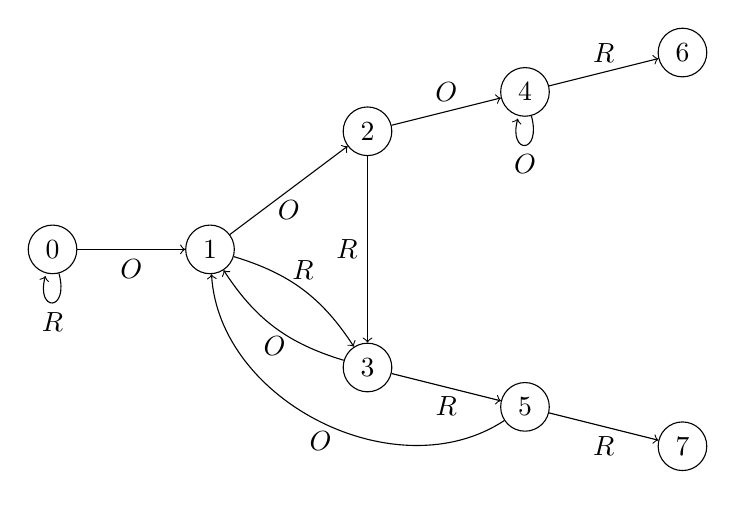
\begin{tikzpicture}[fun/.style={circle, draw=black, minimum size=1}]
  \node[fun] (s) at (0, 0) {$0$};
  
  \path (s) edge [loop below] node [midway, below] {$R$} (s);

  \node[fun] (o1) at (2, 0) {$1$};
  \path[->] (s) edge node [midway, below] {$O$} (o1);

  \node[fun] (o2) at (4, 1.5) {$2$};
  \path[->] (o1) edge node [midway, below] {$O$} (o2);

  \node[fun] (o3) at (4, -1.5) {$3$};
  \path[->] (o1) edge [bend left=20] node [midway, above] {$R$} (o3);
  \path[->] (o3) edge [bend left=20] node [midway, below] {$O$} (o1);
  \path[->] (o2) edge node [midway, left] {$R$} (o3);

  \node[fun] (o4) at (6, 2) {$4$};
  \path[->] (o2) edge node [midway, above] {$O$} (o4);
  \path[->] (o4) edge [loop below] node [midway, below] {$O$} (o4);

  \node[fun] (o5) at (6, -2) {$5$};
  \path[->] (o3) edge node [midway, below] {$R$} (o5);
  \path[->] (o5) edge [bend left=60] node [midway, below] {$O$} (o1);

  \node[fun] (o6) at (8, 2.5) {$6$};
  \path[->] (o4) edge node [midway, above] {$R$} (o6);

  \node[fun] (o7) at (8, -2.5) {$7$};
  \path[->] (o5) edge node [midway, below] {$R$} (o7);
  %\path[->] (o7) edge [bend left=80] node [midway, below] {$O$} (o1);

  \end{tikzpicture}\end{center}

  Alicja wygrywa w wierzchołku $6$ z $\prob$ $1$, a w wierzchołku $8$ wygrywa z $\prob$ równym $0$. Rozpisując to cudeńko jako równanie rekurencyjne, gdzie $P_i$ to prawdopodobieństwo, że będąc w wierzchołku $i$ wygra Alicja, dostajemy:
  $$
    \begin{cases}
      P_6=1\\ 
      P_8 = 0\\ 
      P_4 = \frac{1}{2} P_6 + \frac{1}{2} P_4 \\ 
      P_2 = \frac{1}{2} P_4 + \frac{1}{2} P_3 \\ 
      P_1 = \frac{1}{2} P_2 + \frac{1}{2} P_3 \\ 
      P_3 = \frac{1}{2} P_1 + \frac{1}{2} P_5 \\ 
      P_5 = \frac{1}{2} P_1 + \frac{1}{2} P_8
    \end{cases}
  $$

  Czyli $P_5=\frac{1}{2}P_1$, a 
  $$P_3=\frac{1}{2}P_1+\frac{1}{2}P_5=\frac{1}{2}P_1+\frac{1}{4}P_1=\frac{3}{4}P_1$$
  idąc z tym do $P_1$
  $$P_1=\frac{1}{2}P_2+\frac{1}{2}P_3=\frac{1}{2}P_2+\frac{3}{8}P_1$$
  z $P_4$ dostaniemy
  $$P_4=\frac{1}{2} P_6+\frac{1}{2}P_4=\frac{1}{2}+\frac{1}{2}P_4\implies \frac{1}{2}P_4=\frac{1}{2}\implies P_4=1$$
  i przechodzimy do $P_2$ na chwilę
  $$P_2=\frac{1}{2}P_4+\frac{1}{2}P_3=\frac{1}{2}+\frac{3}{8}P_1$$
  podstawiając z powrotem do $P_1$
  $$P_1=\frac{1}{2}P_2+\frac{3}{8}P_1=\frac{1}{4}+\frac{3}{16}P_1+\frac{6}{16}P_1=\frac{1}{4}+\frac{9}{16}P_1$$
  czyli $\frac{7}{16}P_1=\frac{1}{4}\implies P_1=\frac{4}{7}$, a ponieważ
  $$P_0=\frac{1}{2}P_0+\frac{1}{2}P_1\implies P_1=P_0$$
  to prawdopodobieństwo, że wygra Ala wynosi $\frac{4}{7}$.

\end{solution}
